\section{Risultati}
In questa sezione riportiamo le informazioni riguardanti le esperienze
che abbiamo effettuato: elencheremo le sorgenti dei modelli
d'interesse, come utilizzare la libreria sviluppata per riprodurre le
prove ed analizzeremo il nostro processo di costruzione dell'insieme
$\mathbb{B}$.

\subsection{Modelli biologici studiati}
Da un punto di vista biologico, la maggior parte dei modelli oggetto
dei nostri studi sono riferiti a microorganismi batterici e sono
reperibili in \cite{SymBioCyc} e in \cite{MetExplore} gratuitamente:
quelli che si trovano nel primo riferimento sono stati i primi su cui
abbiamo lavorato, mentre i secondi sono quelli su cui abbiamo
esercitato in modo massivo le nostre implementazioni.

Se si trovassero difficolt\`a nella loro ricerca, le due sorgenti sono
disponibili in \cite{MyJavaImpl}, come descritto nella Sezione
\ref{section:used-tools}. Dopo aver scaricato il repository, i modelli
relativi a \cite{SymBioCyc} si trovano all'interno della cartella
\emph{sbml-test-files}, mentre quelli relativi a \cite{MetExplore}
nell'archivio \emph{sbml-test-files/BioCyc15.0.tar.gz}.

Nelle Figure \ref{fig:ResultViewer-standard-models-overview} e
\ref{fig:ResultViewer-MetExplore-models-overview} riportiamo le
elaborazioni riferite, rispettivamente, ai modelli in \cite{SymBioCyc}
e \cite{MetExplore}: per i primi sono state analizzati 8 modelli
contenenti 1841 metaboliti, per i secondi 165 modelli contenenti 12399
metaboliti.

\begin{figure}
  \centering
  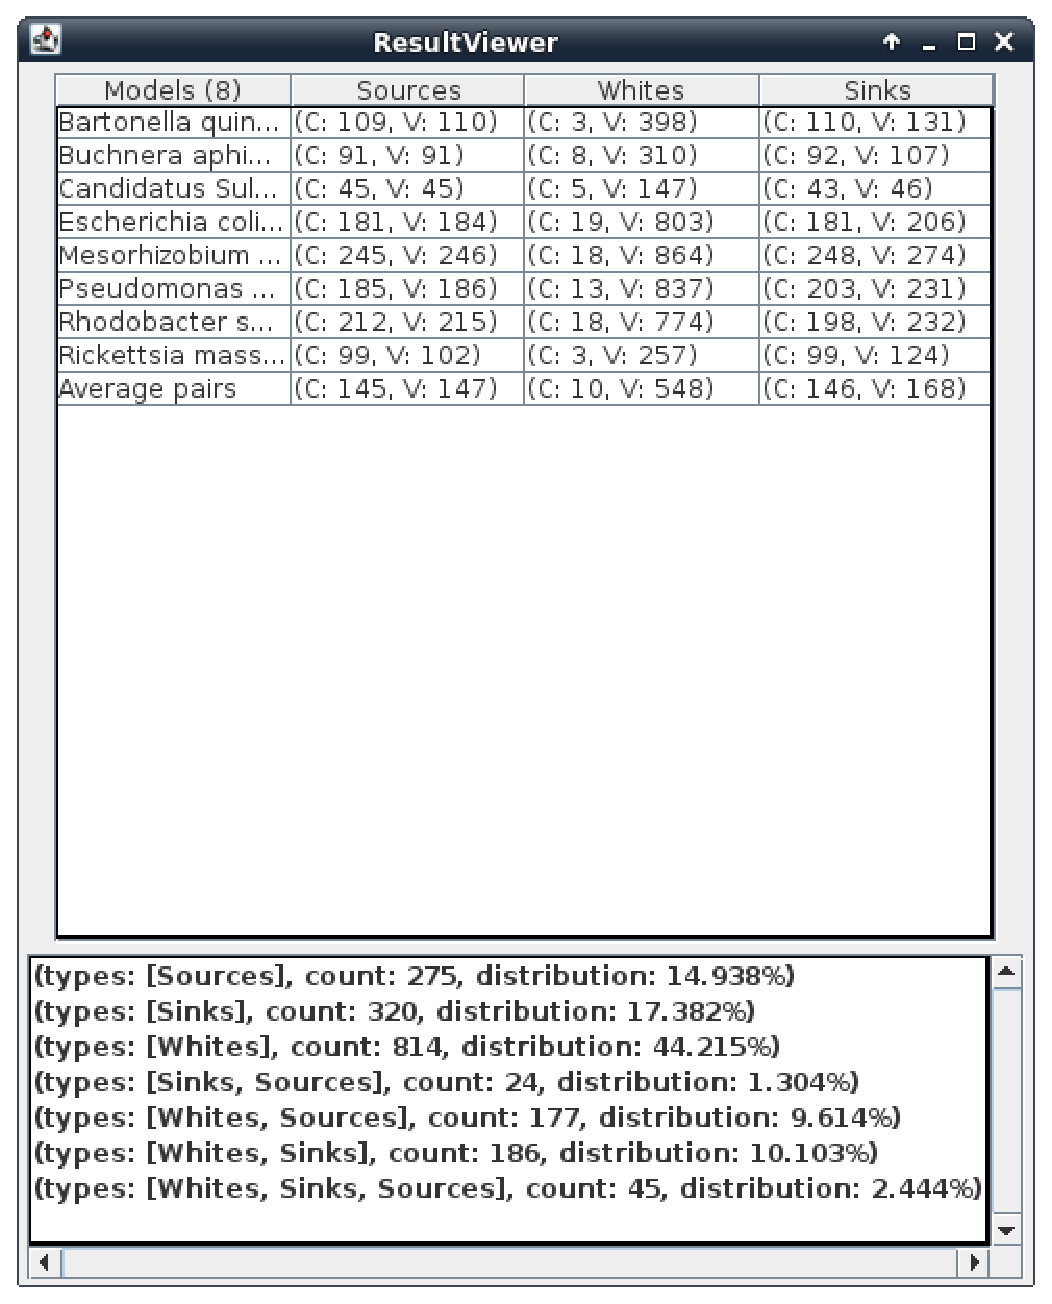
\includegraphics[scale=.7]{images/ResultViewer-standard-models-overview}
  \caption{Panoramica sui modelli in \cite{SymBioCyc}}
  \label{fig:ResultViewer-standard-models-overview}
\end{figure}

\begin{figure}
  \centering
  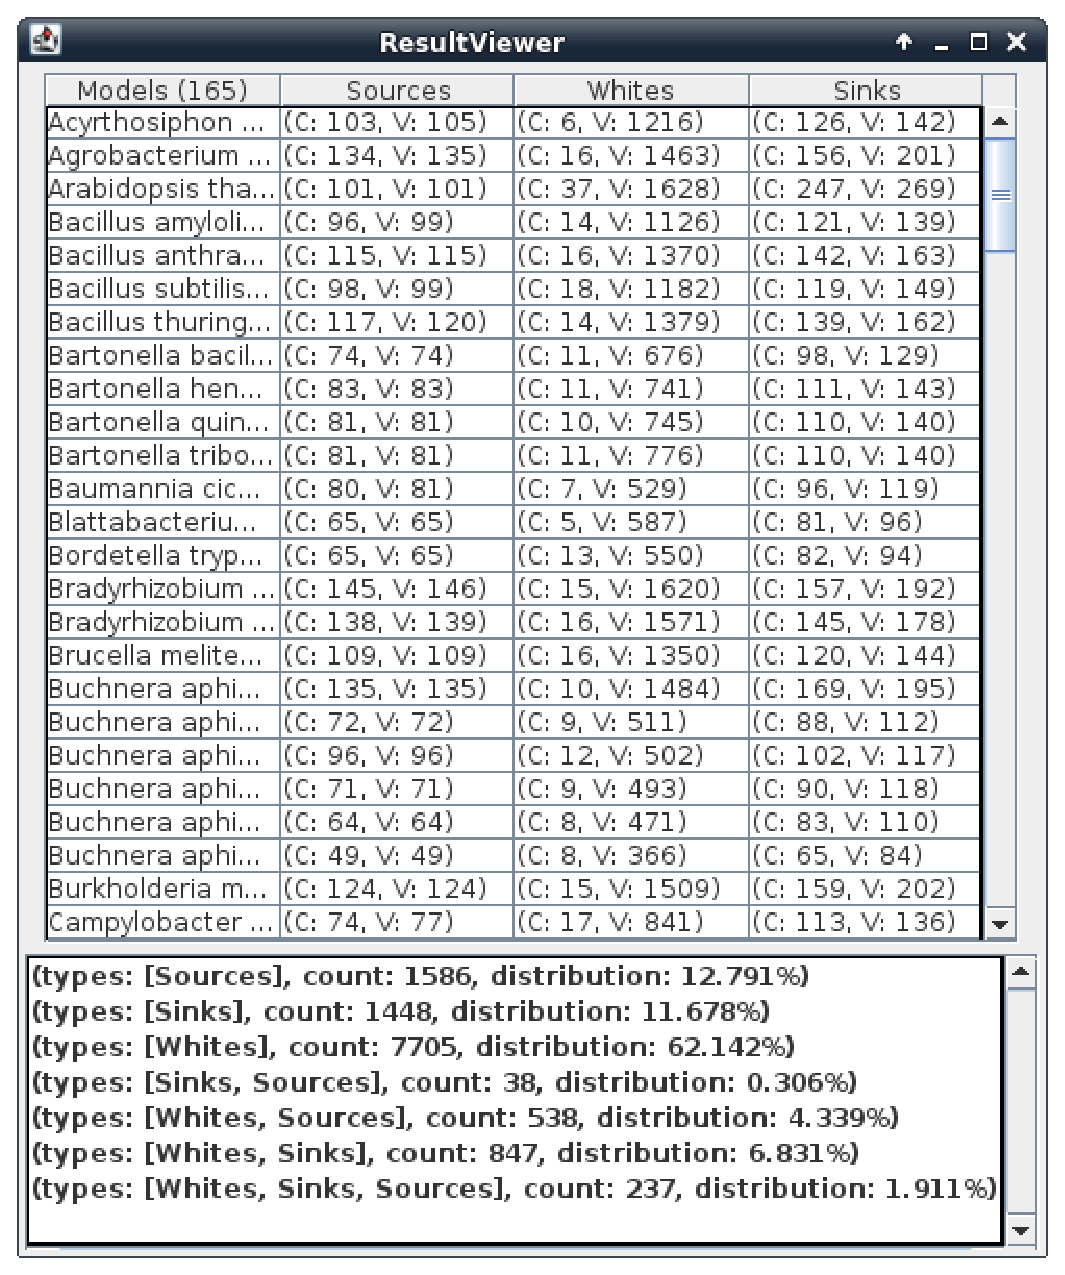
\includegraphics[scale=.7]{images/ResultViewer-MetExplore-models-overview}
  \caption{Panoramica sui modelli in \cite{MetExplore}}
  \label{fig:ResultViewer-MetExplore-models-overview}
\end{figure}


\subsection{Come riprodurre le nostre esperienze}
Ogni prova che abbiamo effettuato \`e codificata in un \emph{metodo di
  test
}, indipendente dalle altre, per cui \`e sufficiente compilare i
sorgenti reperibili in \cite{MyJavaImpl}, sia delle classi che dei
metodi di test, ed esercitare con il \emph{TestRunner} che si
preferisce tutta la batteria di test. I risultati vengono salvati
nella cartella \emph{dot-test-files/tests-output}, all'interno
troviamo:
\begin{itemize}
\item i documenti dot interpretabili con \emph{graphviz} e le relative
  rappresentazioni sotto forma di immagine \emph{svg}, risultato di
  quanto descritto nelle Sezioni
  \ref{subsection:represent-it-in-black-and-white},
  \ref{subsection:apply-depth-first-search} e
  \ref{subsection:use-case-tarjan};
\item i file testuali contenenti informazioni sulla struttura dei
  grafi riferiti sia a dei modelli ``ad hoc'' riportati anche in
  questo documento, sia a reti metaboliche, delle quali non \`e stato
  possibile riportare una rappresentazione data la loro grande
  dimensione. Questi file sono il risultato di quanto descritto nelle
  Sezioni \ref{subsection:tabular-representation-use-case} e
  \ref{subsection:collapse-sources-use-case};
\item le strutture dati contenenti la composizione delle componenti
  fortemente connesse, relative ai modelli presenti nelle sorgenti
  citate nella sezione precedente. Per visualizzarle, usiamo la
  maschera descritta nella Sezione
  \ref{subsection:use-case-result-viewer}, eseguendo la classe
  util.ResultViewer.
\end{itemize}

\subsection{Particolarit\`a di alcuni modelli}
Durante l'esecuzione delle nostre prove abbiamo notato una propriet\`a
che caratterizza alcuni modelli in \cite{MetExplore}: i microorganismi
non sono in biezione con i file in cui sono codificati, bens\`i il
modello di alcuni di loro si ripete in pi\`u di un file con
informazioni diverse. Questa frammentazione dei modelli \`e necessaria
per catturare il concetto di \emph{strain}, che possiamo definire come
una popolazione di microorganismi discendenti da un altro e che sono
leggermente differenti. Per questo motivo abbiamo considerato il
modello contenuto in ogni file indipendente dagli altri: la Figura
\ref{fig:EscherichiaKoli-strains} riporta il microorganismo
\emph{Escherichia coli} e il suo \emph{strain}.
\begin{figure}
  \centering
  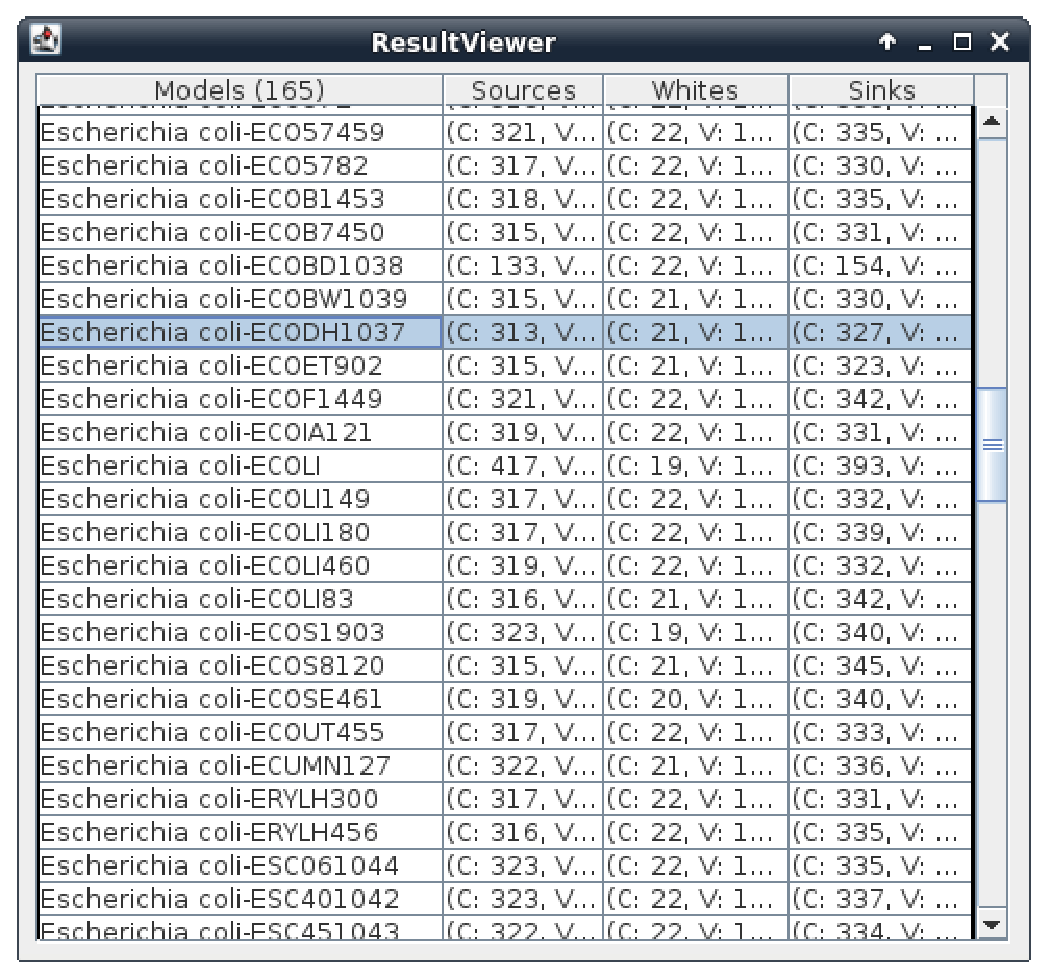
\includegraphics[scale=.7]{images/ResultViewer-Escherichia-family}
  \caption{\emph{Strain} relative al microorganismo \emph{Escherichia
      coli}}
  \label{fig:EscherichiaKoli-strains}
\end{figure}

\subsection{Osservazioni su quanto ottenuto}
Le osservazioni che possiamo fare sui risultati delle prove possono
essere divise in base agli obiettivi che ci poniamo:
\begin{itemize}
\item se si vuole costruire l'insieme $\mathbb{B}$ usando una sola
  rete metabolica allora \`e possibile assegnare un ruolo ad ogni
  metabolito: per visualizzare l'assegnazione \`e sufficiente
  selezionare nella \emph{list-box} alla destra della tabella il ruolo
  e, in risposta, il sistema selezioner\`a, nella rispettiva
  \emph{list-box}, ogni metabolito a cui \`e assegnato il ruolo
  selezionato. Questo \`e il caso proposto nella Figura
  \ref{fig:ResultViewer-single-model} che riporta lo studio del
  modello \emph{Acyrthosiphon}: selezionando la tipologia
  \emph{pozzo}, osservando la selezione nella \emph{list-box} pi\`u in
  basso, possiamo associare tale ruolo ai metaboliti
  \emph{ADP\_IN\_CCO\_45\_IN, ADP\_IN\_CCO\_OUT} e
  \emph{ALL\_45\_TRANS\_45\_...} (oltre a tutti quelli non visibili
  per motivi di spazio) ed includerli nell'insieme $\mathbb{B}$;
  \begin{figure}
    \centering
    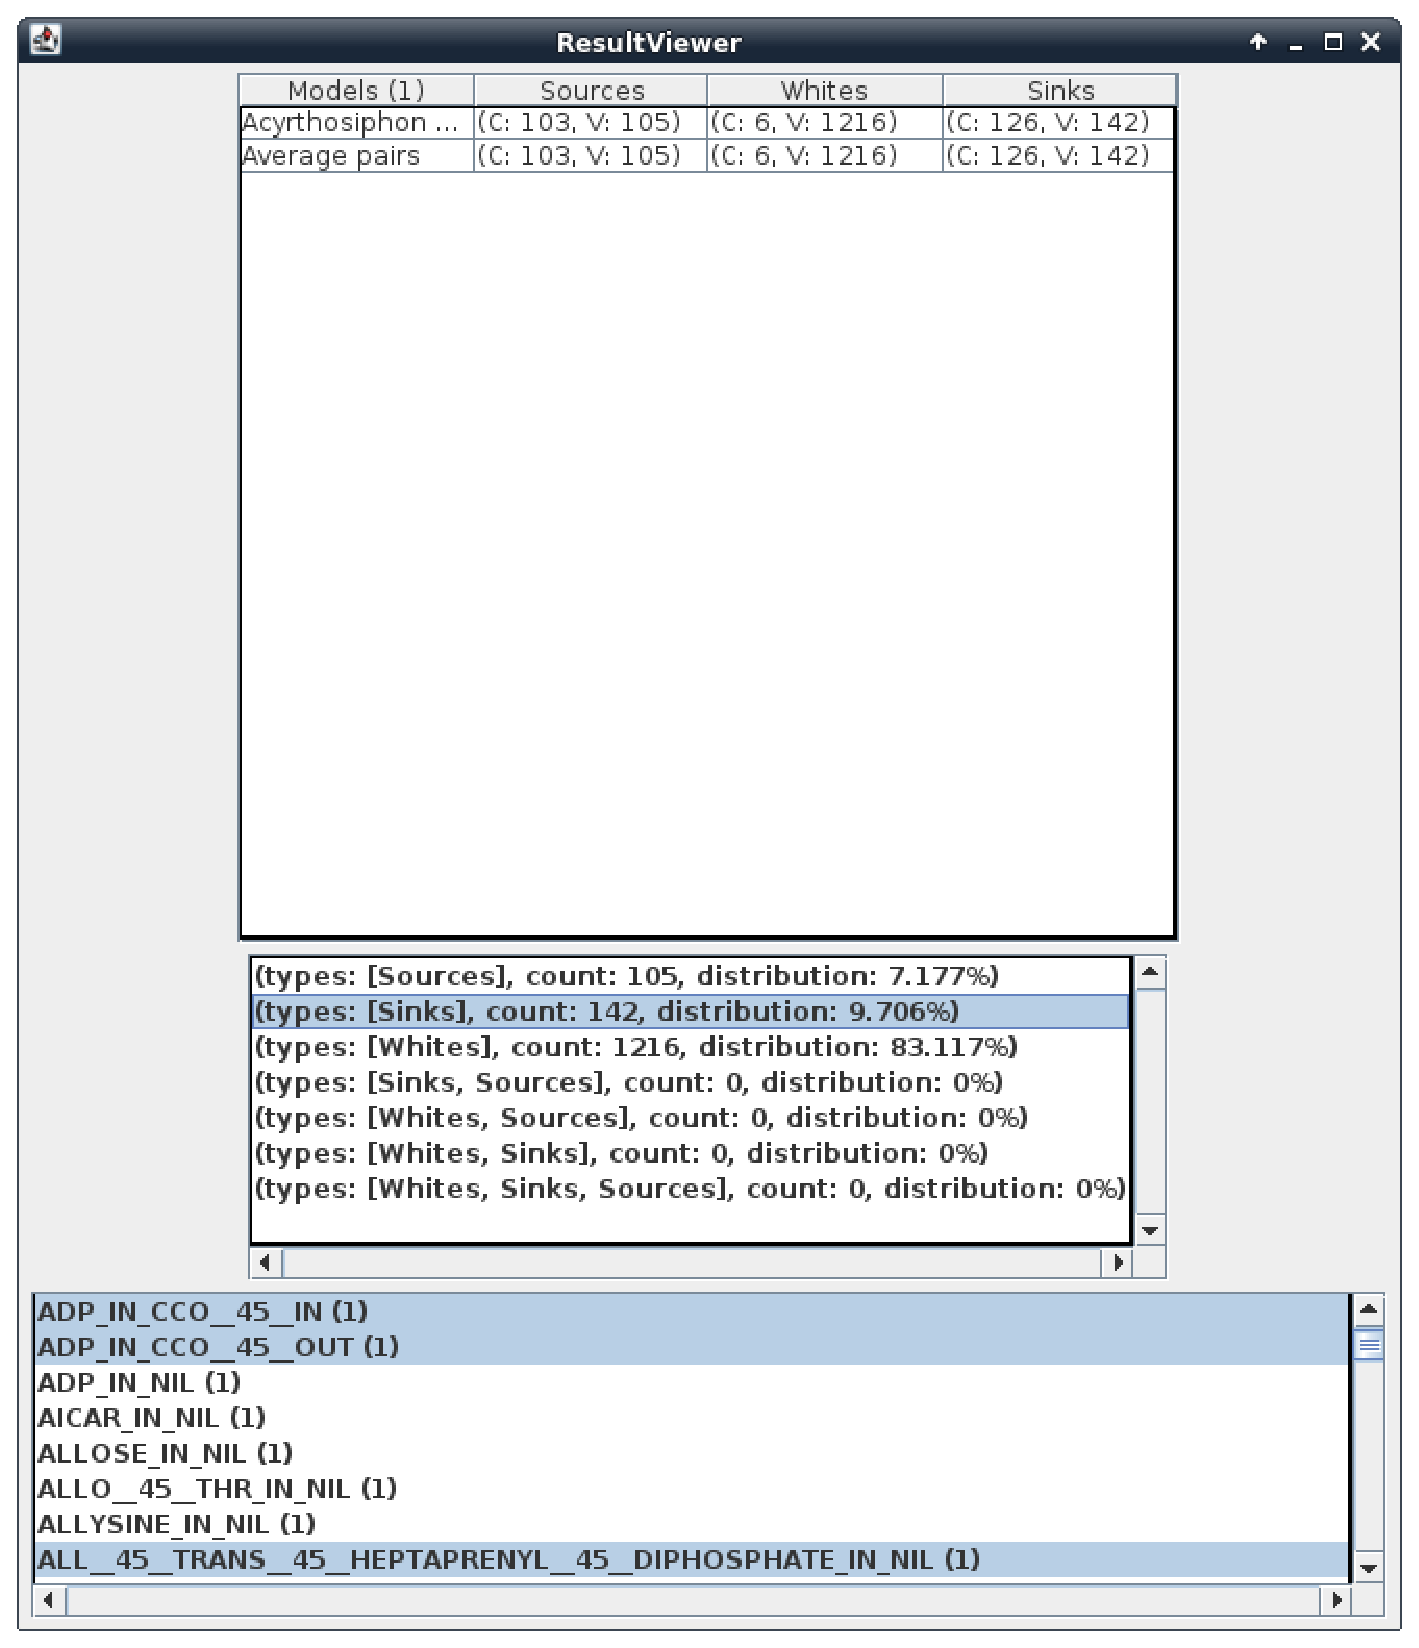
\includegraphics[scale=.6]{images/ResultViewer-single-model}
    \caption{Studio del solo modello \emph{Acyrthosiphon}}
    \label{fig:ResultViewer-single-model}
  \end{figure}

\item se si vuole costruire l'insieme $\mathbb{B}$ usando un insieme
  di reti metaboliche allora si pu\`o avere incoerenza e perdita di
  precisione. Considerando i modelli in \cite{MetExplore} vediamo che
  esistono dei metaboliti che non hanno un singolo ruolo e questo,
  seppur con delle percentuali basse, pu\`o introdurre errori nella
  costruzione dell'insieme $\mathbb{B}$. Questo \`e il caso proposto
  nella Figura \ref{fig:ResultViewer-MetExplore-models}: vediamo che
  esistono 38 metaboliti che, in almeno due modelli, hanno
  rispettivamente il ruolo di pozzo e di sorgente, 538 metaboliti
  invece hanno quello di sorgente e intermedio, ragionando cos\`i per
  gli altri casi arrivando all'ultimo elencato, il quale riporta che
  esistono 237 metaboliti che, in almeno tre modelli, hanno tre ruoli
  diversi. Quest'ultimo caso, insieme alle combinazioni $\{Sources,
  Whites\}$ e $\{Whites, Sinks\}$ (che in totale hanno pi\`u del 10\%
  dei metaboliti totali), produce maggior incertezza in quanto non \`e
  possibile decidere per i 237 metaboliti la loro appartenenza
  all'insieme $\mathbb{B}$;
  \begin{figure}
    \centering
    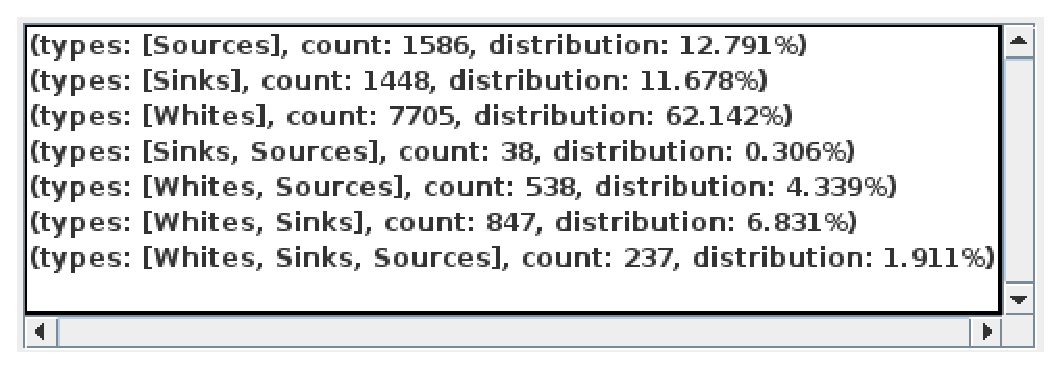
\includegraphics[scale=.7]{images/ResultViewer-grouping-table-zoom}
    \caption{Indagine su tutti i modelli in \cite{MetExplore}}
    \label{fig:ResultViewer-MetExplore-models}
  \end{figure}

\item se si vuole semplificare la rete utilizzando il meta grafo delle
  componenti fortemente connesse osserviamo che, per tutti i modelli
  studiati, non abbiamo un grafo significativo in quanto vi sono molte
  componenti sorgenti e pozzo, mentre sono molto poche le componenti
  intermedie. Questo \`e il caso proposto nella Figura
  \ref{fig:ResultViewer-SCC-composition}: abbiamo selezionato la riga
  che riporta le coppie medie calcolate su tutte le coppie precedenti
  e notiamo che le componenti sorgenti e pozzo non sono composte da
  molti metaboliti, mentre le componenti intermedie lo sono. Inoltre
  il meta grafo non \`e utile per elaborazioni successive per la sua
  topologia a ``clessidra'': vi sono molte componenti sorgenti da cui
  \`e possibile raggiungere poche componenti intermedie, dalle quali
  \`e possibile raggiungere molte componenti pozzo.
  \begin{figure}
    \centering
    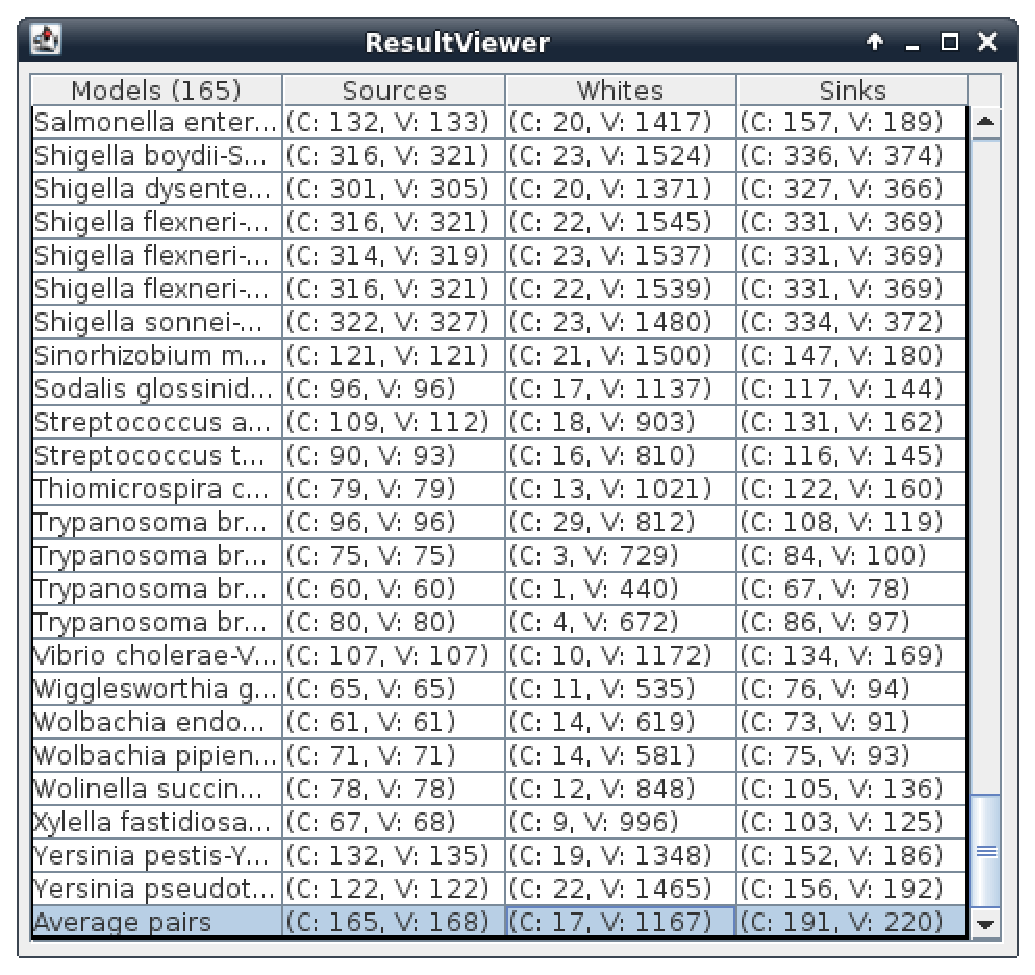
\includegraphics[scale=.7]{images/ResultViewer-table-with-average-row-selected}
    \caption{Numero e cardinalit\`a delle componenti fortemente connesse per i modelli in \cite{MetExplore}}
    \label{fig:ResultViewer-SCC-composition}
  \end{figure}
\end{itemize}
